

\section{Questão 5 - XX = 135} 


\subsubsection{Selecione a trama \textit{beacon} de ordem (260+XX). Esta trama pertence a que tipo de tramas 802.11? Indique o valor dos seus identificadores de tipo e subtipo. Em que parte concreta do cabeçalho da trama estão especificados? (ver anexo)}

    \begin{figure}[H]
    \centering
    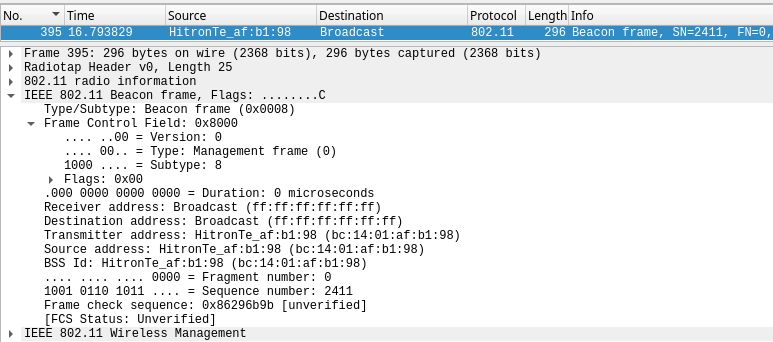
\includegraphics[width=400pt]{Prints/Questao5/questao5-4-trama395.png}
    \caption{Captura da Trama Nº 395.} \label{questao5-1-trama395}
    \end{figure}
    
    
    \par A trama selecionada é a trama de ordem \textbf{395} e pertence ao tipo de tramas \textbf{802.11b (HR/DSSS)}. O campo de tipo tem como valor \textbf{0} que corresponde ao tipo \textit{Management} e o campo de subtipo possui o valor \textbf{8} que corresponde ao subtipo \textit{Beacon}. Estes valores estão especificados dentro dos primeiros dois \textit{bytes} do cabeçalho alusivos à \textit{frame control}, em particular, nos \textit{bits} nº 3-4 (tipo - campo \textit{Type}) e nº 5-8 (subtipo - campo \textit{SubType}) como podemos ver pelo esquema abaixo (cedido pelos docentes):

    \begin{figure}[H]
    \centering
    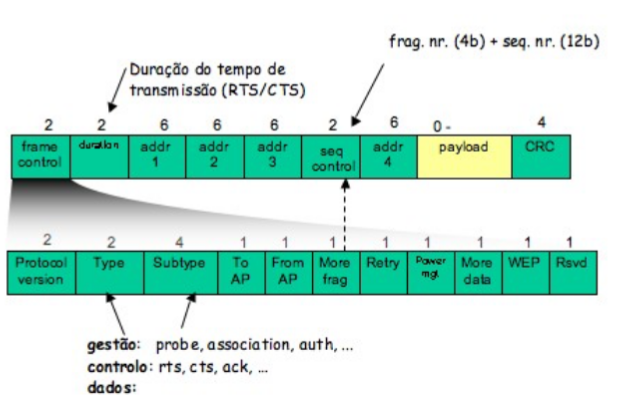
\includegraphics[width=295pt]{Prints/Questao5/stores-anexo.png}
    \label{questao5-1-stores}
    \end{figure}




\newpage
\vspace{20pt}
\subsubsection{Para a trama acima, identifique todos os endereços MAC em uso. Que conclui quanto à sua origem e destino?}

    \vspace{5pt}
    \begin{multicols}{2}
    \begin{itemize}
        \item \textbf{Receiver Address:} ff:ff:ff:ff:ff:ff
        \item \textbf{Destination Address:} ff:ff:ff:ff:ff:ff
        \item \textbf{Transmitter Address:} bc:14:01:af:b1:98
        \item \textbf{Source Address:} bc:14:01:af:b1:98
    \end{itemize}
    \end{multicols}
    
    \vspace{10pt}    
    \par Pela análise da trama, denotamos que tem como origem (\textit{Source} e \textit{Transmitter Address}) um endereço MAC válido (relativo ao AP). O AP envia periodicamente tramas \textit{beacon} para anunciar a sua presença e transmitir informações a todas as interfaces rádio que estão dentro do seu alcance, daí o campo do endereço destino (\textit{Receiver} e \textit{Destination Address}) possuir o endereço com o valor ff:ff:ff:ff:ff:ff que corresponde a uma trama de \textit{broadcast}.







\subsubsection{Uma trama \textit{beacon} anuncia que o AP pode suportar vários débitos de base, assim como vários débitos adicionais (\textit{extended supported rates}). Indique quais são esses débitos?}
    
    \par A partir do campo \textit{Tagged Parameters}, conseguimos denotar tanto os débitos base (\textit{Supported Rates}) como os débitos adicionais (\textit{Extended Rates}) suportados pelo AP.
    
    
    \begin{figure}[H]
    \centering
    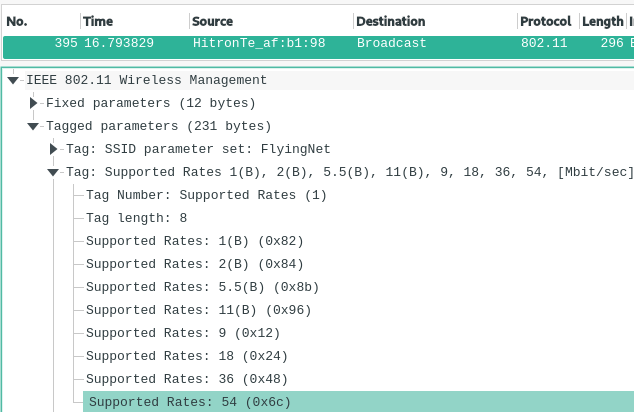
\includegraphics[width=250pt]{Prints/Questao5/questao5-VariousRates.png}
    \caption{AP \textit{\textbf{Supported} Rates}.} \label{questao5-SuppRates}
    \end{figure}

    \begin{figure}[H]
    \centering
    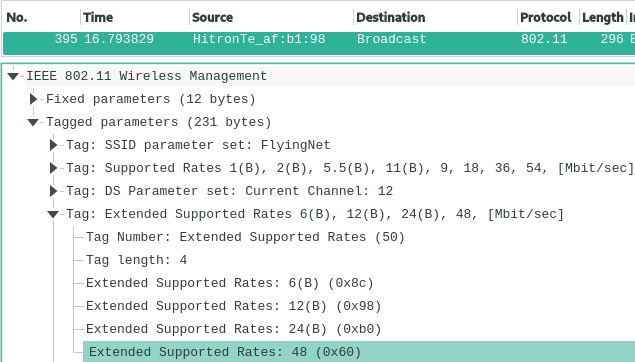
\includegraphics[width=250pt]{Prints/Questao5/questao5-VariousRates-Extended.png}
    \caption{AP \textit{\textbf{Extended} Rates}.} \label{questao5-ExtRates}
    \end{figure}
        
        





\subsubsection{Qual o intervalo de tempo previsto entre tramas \textit{beacon} consecutivas (este valor é anunciado na própria trama \textit{beacon})? Na prática, a periodicidade de tramas \textit{beacon} provenientes do mesmo AP é verificada com precisão? Justifique.}

    \par O valor do intervalo de tempo previsto entre tramas \textit{beacon} consecutivas é anunciado na própria trama \textit{Beacon}, estando presente no campo \textit{\textbf{Beacon Interval}}, neste caso, com o valor de \textbf{0.1024 segundos}. No entanto, este valor, apesar de estar definido na trama, pode não ser respeitado com precisão, podendo haver atrasos ou adiantamentos, uma vez que os tempos de transmissão do AP podem variar de acordo com a sua "carga"\xspace de transmissão no momento.
    
    \begin{figure}[H]
    \centering
    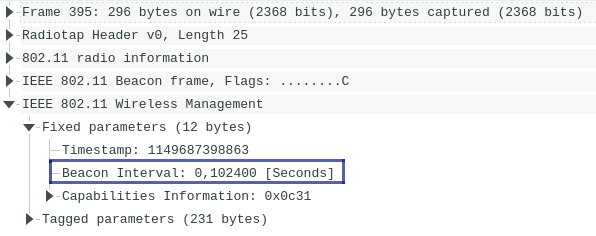
\includegraphics[width=300pt]{Prints/Questao5/questao2-IntervTempo.png}
    \caption{Intervalo de Tempo tramas \textit{Beacon}.} \label{questao5-InterTempo}
    \end{figure}




\vspace{15pt}
\subsubsection{Identifique e liste os SSIDs dos APs que estão a operar na vizinhança da STA de captura? Explicite o modo como obteve esta informação (por exemplo, se usou algum filtro para o efeito).}

    \par Para obtermos os SSIDs que estão a operar na vizinhança da STA de captura, tivemos de desenvolver um filtro a aplicar na ferramenta \textit{Wireshark}. Assim, como sabemos que o tipo de tramas utilizadas pelos APs para anunciar a sua presença são as tramas \textit{Beacon} e o seu valor é 8 (já consultado nas alíneas anteriores), aplicamos o seguinte filtro:
    
    \vspace{10pt}
    \begin{minipage}{\linewidth}
        \centering
        \fbox{ wlan.fc.type\_subtype $==$ 0x08  }
    \end{minipage}

    \vspace{10pt}
    \par De seguida, obtivemos o seguinte resultado notando várias tramas que obedecem ao filtro, mas apenas dois SSID's distintos na vizinhança: \textbf{FlyingNet} e \textbf{NOS\_WIFI\_Fon}. 

    \begin{figure}[H]
    \centering
    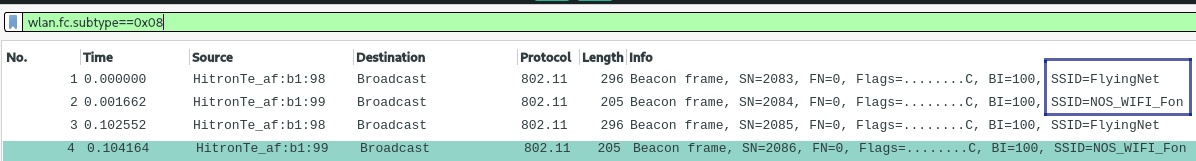
\includegraphics[width=\linewidth]{Prints/Questao5/questao5-SSID.png}
    \caption{SSIDs na vizinhança da STA de captura.} \label{questao5-SSID}
    \end{figure}
    
    \par Conseguimos confirmar que apenas existem estes dois SSIDs uma vez que quando adicionamos as seguintes condições ao filtro acima, o resultado foi vazio: 
    
    \vspace{5pt}
    \begin{minipage}{\linewidth}
    \centering
    \fbox{ ... \&\& (wlan.ssid != NOS\_WIFI\_Fon) \&\& (wlan.ssid != FlyingNet)}
    \end{minipage}







\subsubsection{Verifique se está a ser usado o método de deteção de erros (CRC). Justifique o porquê de ser necessário usar deteção de erros em redes sem fios.}
    
    \par O campo \textit{\textbf{Frame Check Sequence}} (FCS) é utilizado para verificar a integridade do pacote do lado que a recebe. O recetor analisa e calcula o valor CRC correto do pacote, comparando de seguida com o valor que realmente veio na trama. Assim, se os valores não coincidirem, o pacote é considerado corrumpido. Neste caso em particular, para obtermos as várias tramas \textit{beacon} WLAN possivelmente corrumpidas, aplicamos o filtro fornecido pelos docentes:
        
    \vspace{10pt}
    \begin{minipage}{\linewidth}
    \centering
    \fbox{ (wlan.fc.type\_subtype $==$ 0x08)  \&\&  (wlan.fcs.status $==$ bad) }
    \end{minipage}
   
    \vspace{10pt}
    \par No entanto, apesar do filtro estar bem construído não obtivemos qualquer resultado de tramas capturadas que obedecessem ao mesmo (Figura \ref{questao5-CRC-Empty}). Para além disto, notamos que caso apenas aplicássemos a primeira parte do filtro (\textit{wlan.fc.type\_subtype $==$ 0x08}), obtínhamos tramas que, ao analisarmos o conteúdo da mesma, continham o valor \textit{unverified} no campo FCS (Figura \ref{questao5-CRC-1}), não podendo tirar conclusões sobre a utilização do método de deteção de erros CRC.
    
    \vspace{10pt}
    \begin{minipage}{0.5\linewidth}
    \centering
        \begin{figure}[H]
        \centering
        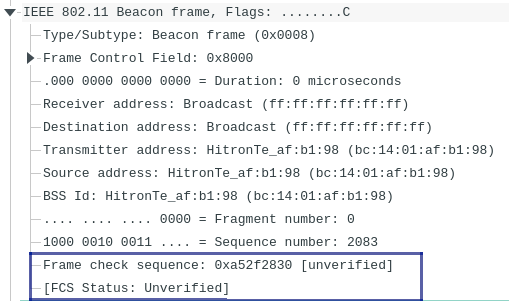
\includegraphics[width=\linewidth]{Prints/Questao5/questao5-CRC-1.png}
        \caption{Primeira captura.} \label{questao5-CRC-1}
        \end{figure}
    \end{minipage}
     \begin{minipage}{0.5\linewidth}
        \centering
        \begin{figure}[H]
        \centering
        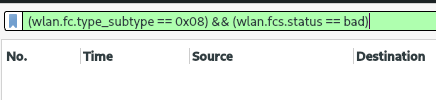
\includegraphics[width=\linewidth]{Prints/Questao5/questao5-CRC-Empty.png}
        \caption{Resultado do filtro completo.} \label{questao5-CRC-Empty}
        \end{figure}
    \end{minipage}  
  
    \vspace{15pt}
    Após uma pesquisa \textit{online} sobre a ferramenta \textit{Wireshark}, descobrimos que esta opção estaria desativada. Como tal, ativamos a opção seguindo os passos encontrados neste site: \href{http://wifinigel.blogspot.com/2019/11/wireshark-showing-fcs-fields-as.html}{Enabling FCS}. Voltamos a analisar o tráfego capturado, inserindo o filtro completo mas voltamos a obter um resultado vazio. Assim, atribuímos o não obtermos tramas \textit{beacon} corrumpidas a mau funcionamento da ferramenta ou da captura, uma vez que quando apenas aplicamos a segunda parte do filtro, ou seja, filtrar quaisquer tramas corrumpidas, o \textit{Wireshark} consegue apresentar resultados.
  
    \vspace{5pt}
    \par Uma vez que redes \textit{Wi-Fi} se propagam pelo meio (sem fios), estas são propícias a erros, pois estão vulneráveis a interferências como obstáculos que não consigam ultrapassar ou que provoquem distorção no conteúdo transmitido. Como tal, a utilização de métodos de deteção de erros é fulcral para evitar falhas na transmissão de tramas, uma vez que uma mudança em apenas um \textit{bit} pode ter como consequência a corrupção do pacote. 
    
    





\newpage
\subsubsection{Estabeleça um filtro \textit{Wireshark} apropriado que lhe permita visualizar todas as tramas \textit{probing request} e \textit{probing response}, simultaneamente.}

    \par De forma a restringir a procura de tramas \textit{probing request} e \textit{response}, apenas nos bastou aplicar o filtro ao campo do subtipo da trama, isto é, igualar o tipo e subtipo aos seus valores devidos em hexadecimal: \textbf{0x04} (\textit{management probe request}) e \textbf{0x05} (\textit{management probe response}).

    \vspace{10pt}
    \begin{minipage}{\linewidth}
        \centering
        \fbox{
        (wlan.fc.type\_subtype $==$ 0x04) \space\space \textbf{or} \space\space (wlan.fc.type\_subtype $==$ 0x05)
        }
    \end{minipage}

    \vspace{10pt}
    \par De forma a verificarmos o bom funcionamento do filtro apresentamos um \textit{print} do seu resultado na ferramenta \textit{Wireshark}, onde captamos ambos os tipos de tramas:
    
    \begin{figure}[H]
    \centering
    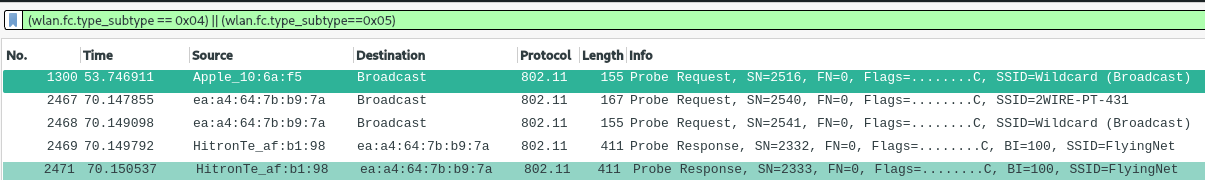
\includegraphics[width=\linewidth]{Prints/Questao5/questao5-ReqRespnse.png}
    \caption{Resultado da aplicação do filtro.} \label{questao5-ReqResponse}
    \end{figure}
    




\vspace{10pt}
\subsubsection{Identifique um \textit{probing request} para o qual tenha havido um \textit{probing response}. Face ao endereçamento usado, indique a que sistemas são endereçadas estas tramas e explique qual o propósito das mesmas?}

    \par Para conseguirmos obter um par \textit{probing response} e \textit{probing request}, tivemos de analisar os endereços das tramas e procurar uma correspondência, ou seja, para o endereço destino de \textit{Response}, encontrar um \textit{Request} que possua esse endereço no campo origem. Obtivemos o seguinte par:
    
    \begin{figure}[H]
    \centering
    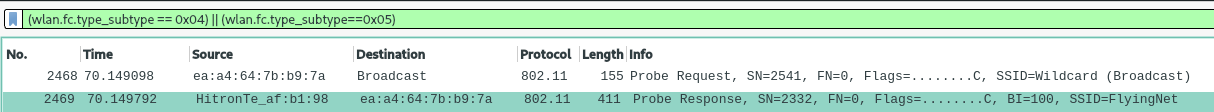
\includegraphics[width=\linewidth]{Prints/Questao5/questao5-PAR.png}
    \caption{Par \textit{Resquest}-\textit{Response}.} \label{questao5-PARreqResp}
    \end{figure}
    
    \par Analisando o conteúdo das tramas, conseguimos denotar que a trama correspondente ao \textit{Probing Request} possui como endereço MAC de origem \textbf{ea:a4:64:7b:b9:7a} e como destino \textbf{ff:ff:ff:ff:ff:ff}, concluindo que se trata de uma trama de \textit{broadcast}, tendo como origem um dispositivo com interesse em ligar-se a uma rede. Relativamente à trama de \textit{Probing Response}, esta possui o endereço MAC de origem com o valor \textbf{bc:14:01:af:b1:98} e como endereço destino o endereço \textbf{ea:a4:64:7b:b9:7a}, conferindo assim a propriedade referida acima sobre a correspondência de endereços.
    
    \par Assim, estas tramas servem para que dispositivos se consigam ligar a redes, através de pedidos (\textit{requests}) e respostas dos APs (\textit{response}). Neste caso em particular, o dispositivo interessado em conectar-se, recebeu do AP não só o endereço MAC do mesmo como também o SSID da rede que o AP é responsável.